\documentclass[12pt]{article} % article class, 12pt font

% load any packages you need for more custom stuff
\usepackage[margin=1in]{geometry} % set 1-inch margins
%\usepackage{setspace}\doublespacing % set double spacing
\usepackage[superscript]{cite} % superscript numeric in-line citations
\usepackage[spanish]{babel} 
\usepackage[utf8]{inputenc}
\usepackage{indentfirst} % indent the first paragraph of each section
\usepackage{hyperref}
\hypersetup{
    colorlinks=true,
    linkcolor=blue,
    filecolor=magenta,      
    urlcolor=cyan,
}

% set title stuff
\title{Perfil personal}
\newcommand{\authors}{}
\author{Diego Quirós Artiñano}\date{\today} 

% start the actual document
\usepackage{graphicx}
\begin{document}

% create title stuff
\hfill\authors % write the authors right-aligned
\vspace{-0.25in} % reduce space before title
{\let\newpage\relax\maketitle} % print title
\vspace{-0.1in} % reduce space after title



\begin{figure}[htp]
\centering
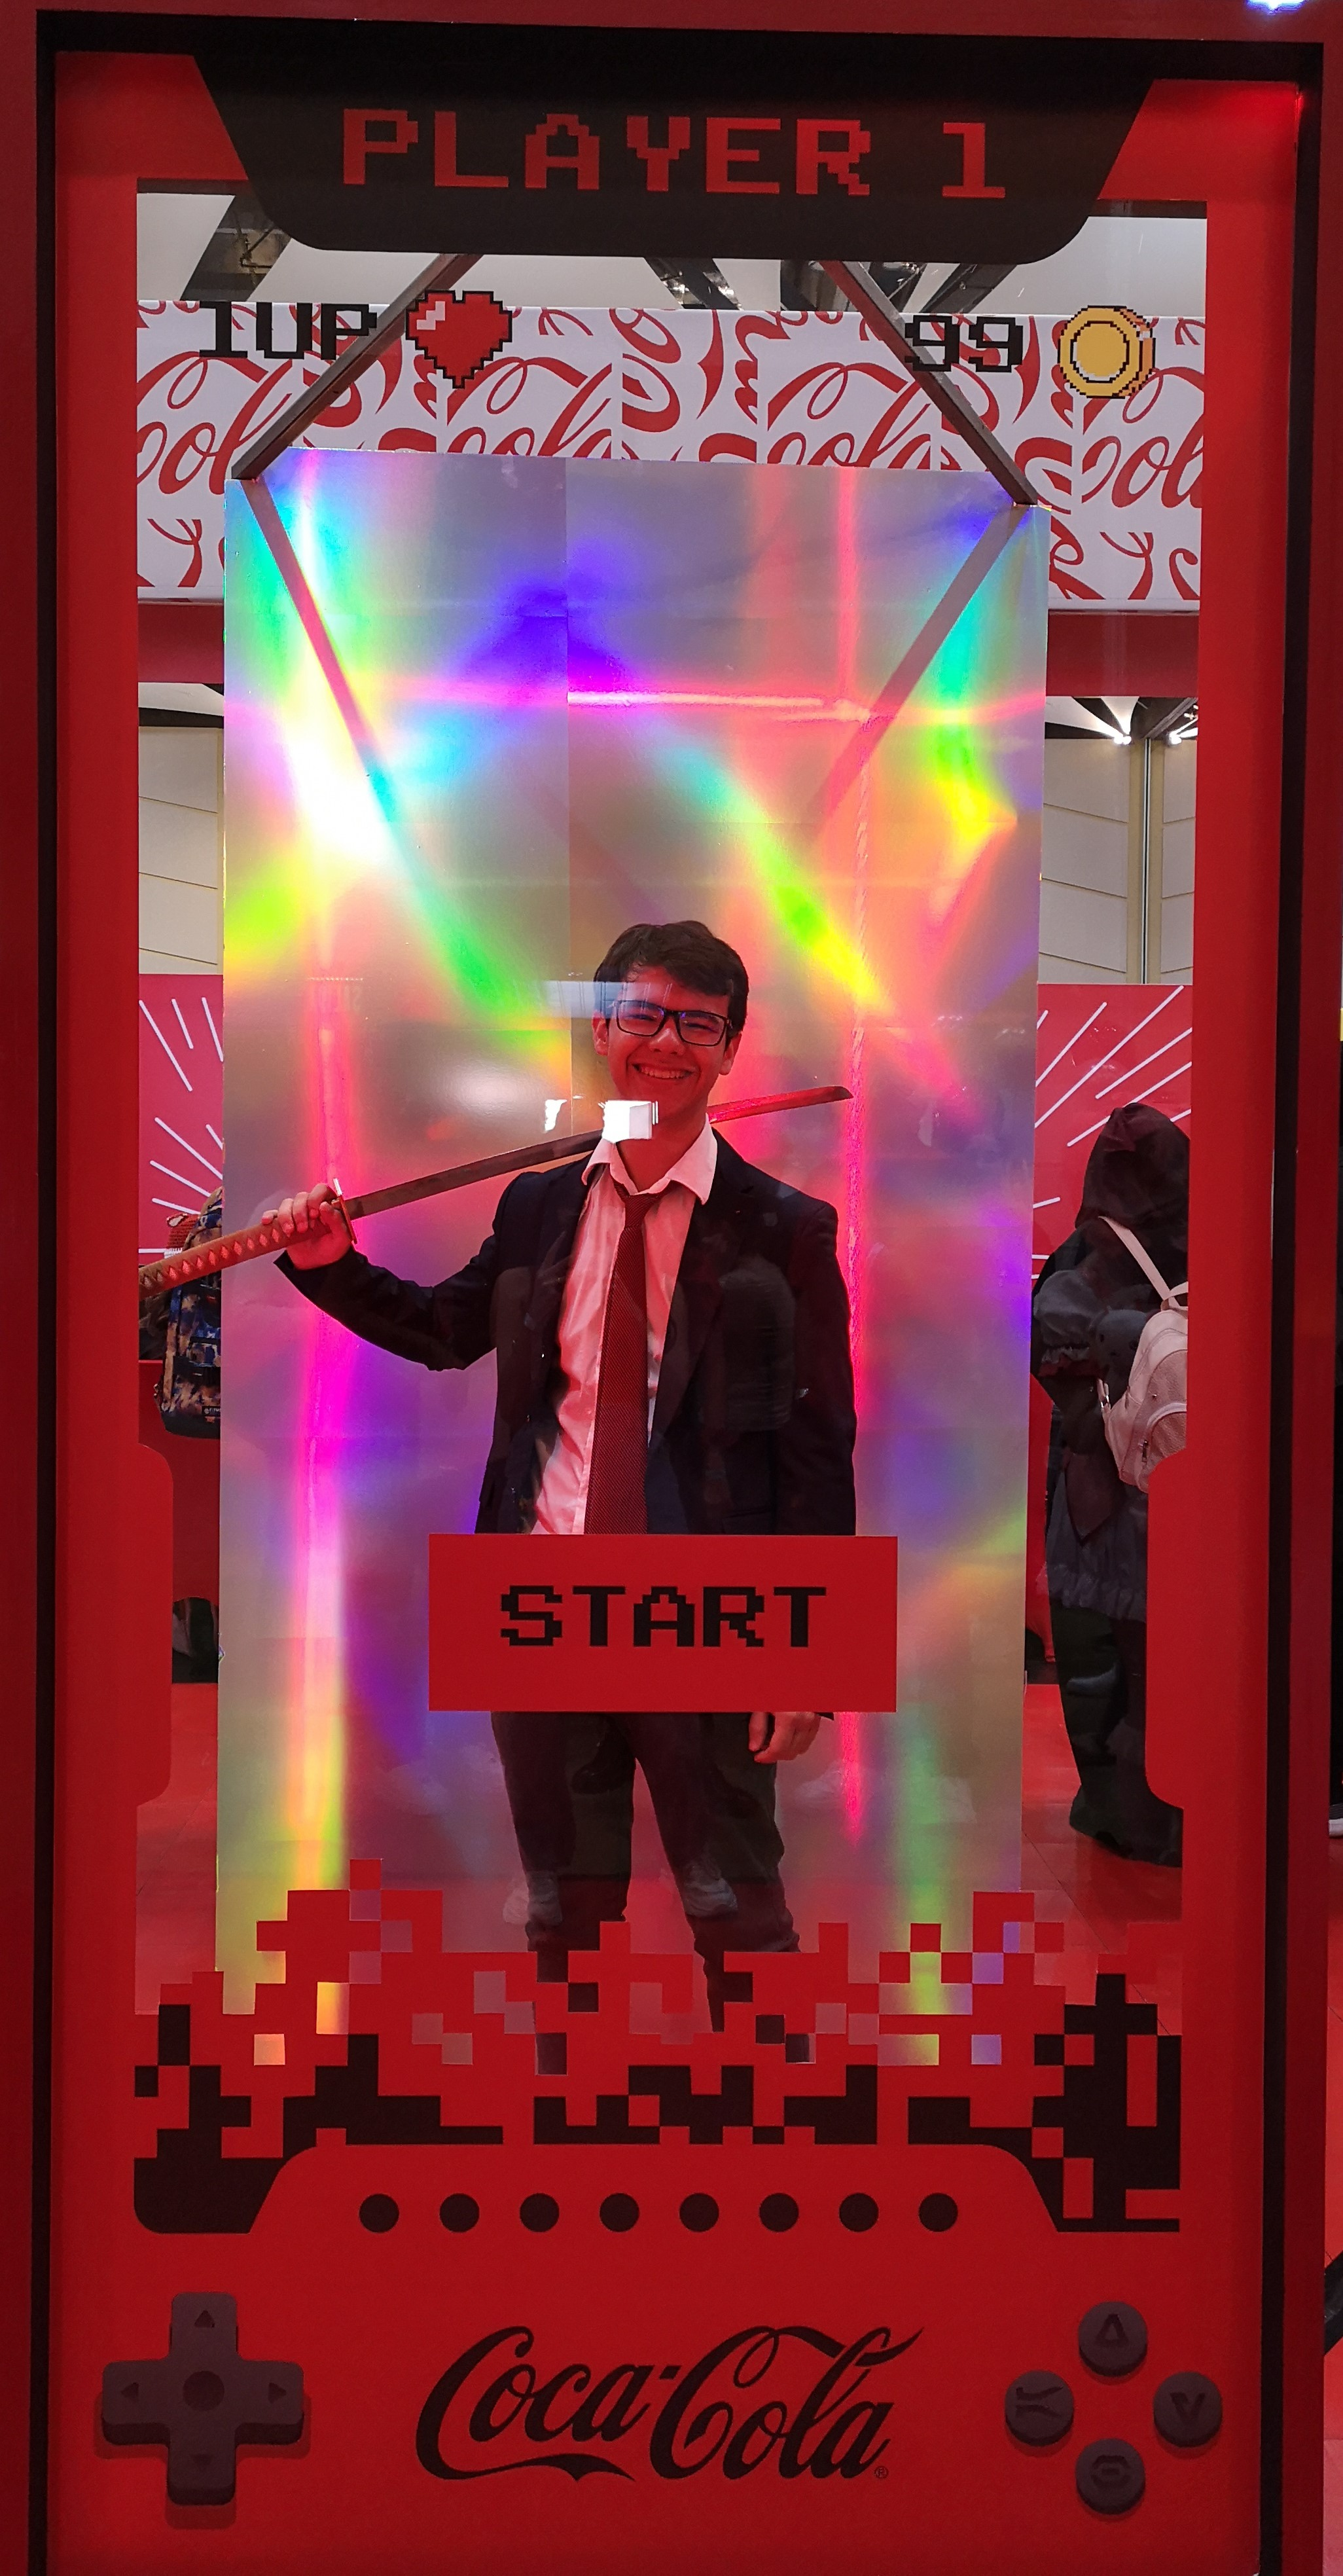
\includegraphics[scale=0.15]{./FotosPerfil/Connecturday1Cropped.jpg}
% 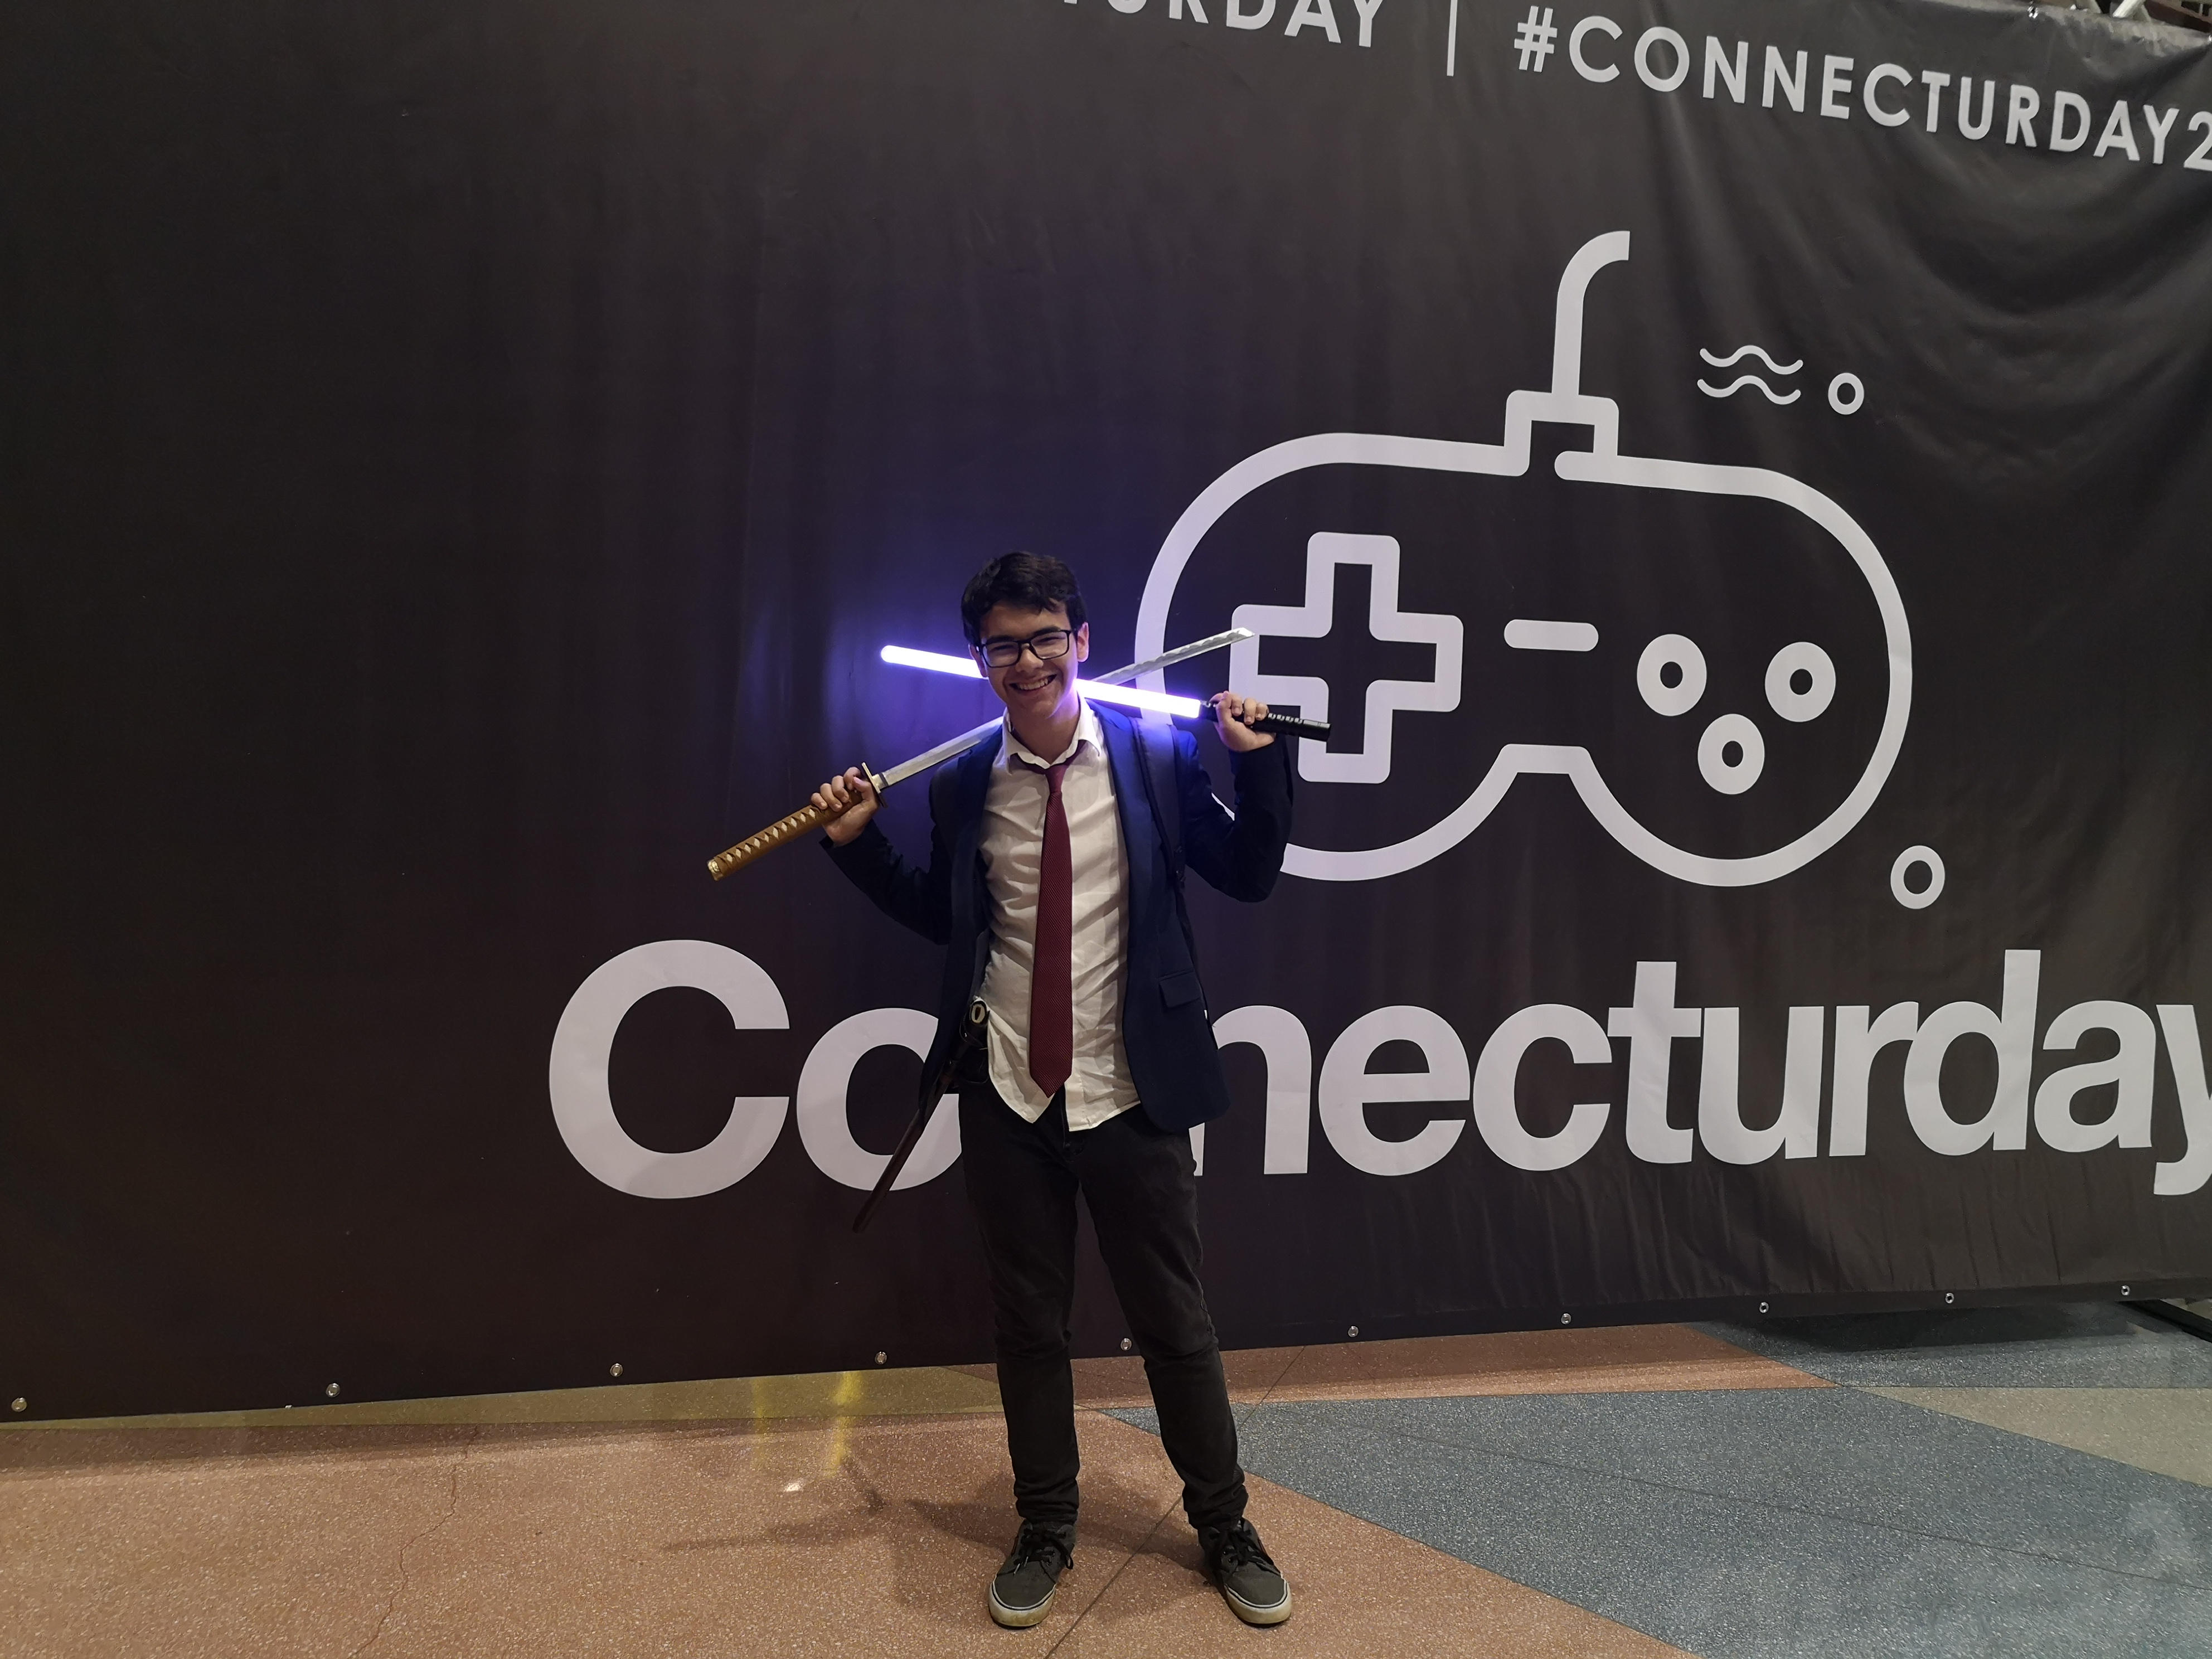
\includegraphics[scale=0.12]{./FotosPerfil/Connecturday2.jpg}
% 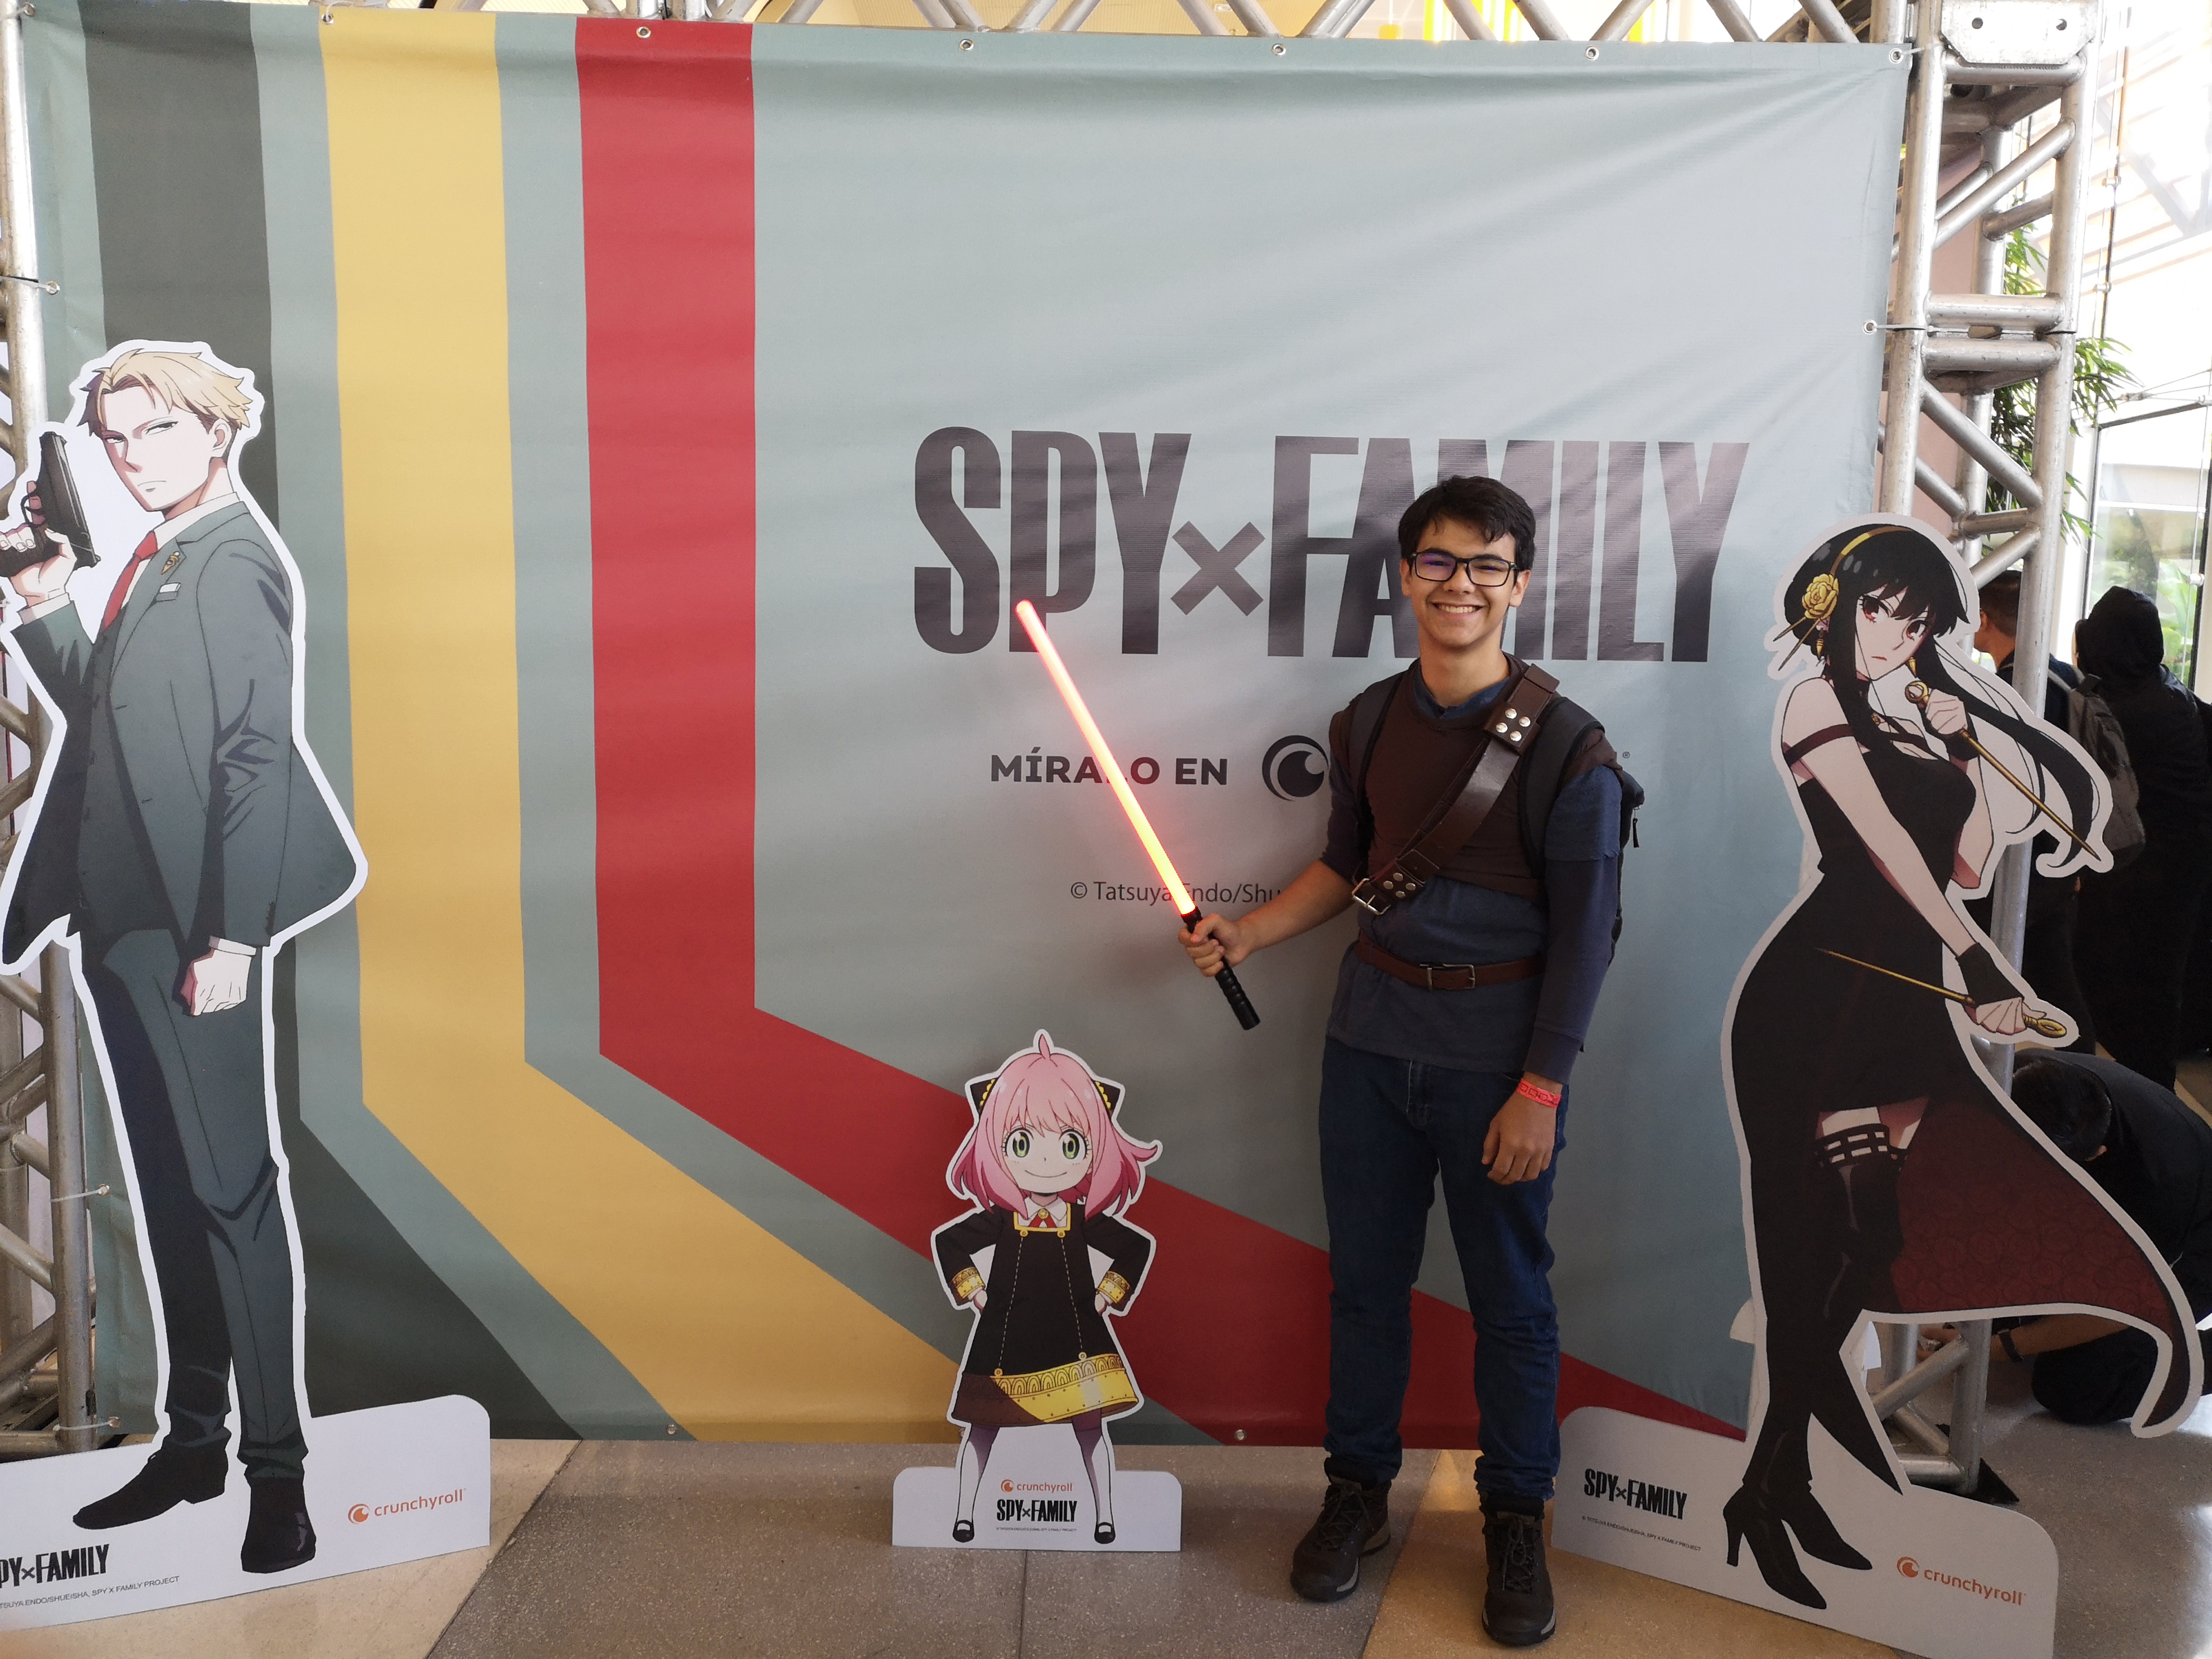
\includegraphics[scale=0.12]{./FotosPerfil/Connecturday3.jpg}
% \includegraphics[scale=0.08]{./FotosPerfil/TesoroEscondido2.jpg}
% \includegraphics[scale=0.08]{./FotosPerfil/TesoroEscondido1.jpg}
% \includegraphics[scale=0.11]{./FotosPerfil/TesoroEscondido4.jpg}

\caption{}
\label{foto}
\end{figure}

% begin the main text
\section*{Mini-biografía}
Soy un estudiante que le encanta el reto. Las pruebas dificiles siempre me han parecido chvisimas, razón por la que asistí todos los años que pude en OLCOMA durante el colegio (aunque nunca pasara de la segunda ronda). Desde pequeño supe que me gustaba la tecnología, era el que colocaba los cables en sus colores respectivos para que sirviera el VHS o reproductor de DvDs. En el momento que pude matriculé el curso de Programación en el cole, donde vimos un poco de Java, tras de eso supe que esa area es en la que me gustaría desarrollarme, tanto que pedí que me abrieran el curso de netacad de Python. A pesar de eso, igualmente me informé con todos los exámenes de personalidad y aptitud que me podían hacer, todos me terminaron diciendo que me debería dedicar a las ingenierías, excepto por un ''outlier'' que decía que tenía aptitud para artes. Si algo me causa curiosidad de aprender casí que imediatamente me pongo a buscar, razón por la cual mi familia odia ver peliculas conmigo, porque de la nada tengo un montón de datos de los actores que a nadie más le interesa.

Yo soy graduado de Blue Valley School y estudiante regular en la UNA. 


\section*{Hobbies}

\begin{itemize}
\item \textbf{}:
\end{itemize}


\section*{Películas favoritas}

\begin{itemize}
\item \textbf{}:
\end{itemize}

\section*{Libros favoritos}

\begin{itemize}
\item \textbf{} ():
\end{itemize}

\section*{Frases favoritas}

\begin{itemize}
\item \textit{} \textbf{}
\end{itemize}

\section*{Planes a futuro}

\begin{itemize}
\item 
\end{itemize}

\section*{Expectativa del curso}
% En esta sección espero que me indiquen cuál es la expectativa del curso y si pueden, de la carrera.


\section*{¿Algo más?}
%personas que les inspiran, si les gustan los animales, cualquier cosa que quieran agregar... ¿qué espera del curso?

\section*{¿Qué es un buen profesor?}

\end{document} % this ends your document